\documentclass[wide,a4paper,titlepage,12pt] {article}
\usepackage{polski}
\usepackage[utf8]{inputenc}
\usepackage{listings}
\usepackage{slashbox}
\usepackage[table]{xcolor}
\usepackage{graphicx,pdflscape}
\usepackage{placeins}


\title{Projektowanie efektywnych algorytmów}
\author{Tymon Tobolski (181037)}

% Title page layout (fold)
\makeatletter
\renewcommand{\maketitle}{
\begin{titlepage}
  \begin{center}
    \vspace*{3cm}
    \LARGE \@title \par
    \vspace{2cm}
    \textit{\small Autor:}\par
    \normalsize \@author\par \normalsize
    \vspace{3cm}
    \textit{\small Prowadzący:}\par
    Mgr inż. Karolina Mokrzysz \par
    \vspace{2cm}
    Wydział Elektroniki\\ III rok\\ Pn TP 11.15 - 1.00\par
    \vspace{4cm}
    \small \@date
  \end{center}
\end{titlepage}
}
\makeatother
  \lstset{
    language=haskell,
    basicstyle=\ttfamily\scriptsize,
    numbers=left,
    numberstyle=\scriptsize,
    stepnumber=10,
    numbersep=9pt,
    showspaces=false,
    showstringspaces=false,
    showtabs=false,
    breaklines=true,
  }

\begin{document}
\maketitle
  \section{Opis problemu}
  \paragraph{}
  Dla podanej listy zadań znaleźć najbardziej optymalne uszeregowanie,
  minimalizujące opóźnienia.

  \paragraph{}
  Każde zadanie posiada określony czas wykonania ($p$),
  czas w którym powinno być wykonane ($d$) oraz wagę ($w$).
  W przypadku gdy zadanie jest zostało wykonane do czasu $d$ naliczane jest opóźnienie.
  Celem algorytmu jest takie uszeregowanie zadań, aby suma kosztów opóźnień wszystkich zadań
  była jak najmniejsza. Koszt opóźnienia zadania wyraża się wzorem:

  $l(t) = w * max(0, t - d) $

  \section{Opis algorytmu}
  \paragraph{}
  Dla opisanego problemu zostały sprawdzone trzy wersje algorytmu szeregującego.

  \subsection{Przegląd zupełny}
  Przegląd zupełny polega na sprawdzeniu każdej możliwej permutacji list zadań,
  policzeniu koszty każdej z nich, a następnie wybranie tej o najmniejszym koszcie.


  \subsection{Pierwsza procedura eliminacyjna}
  \paragraph{}
  Jednym ze sposobów ulepszenia przeglądu zupełnego jest obliczanie na bieżąco
  kosztu rozwiązania częściowego i porównanie go z dotychczasowym najmniejszym
  kosztem. W przypadku gdy jego koszt jest większy niż najmniejszy obecny, rozwiązanie
  takie zostaje odrzucone wraz ze wszystkimi rozwiązaniami, które powstały by w przypadku
  kontunuacji permutacji. W przypadku gdy koszt jest mniejszy następuje dalsze sprawdzanie
  rozwiązań, a koszt tego rozwiązania częsciowego zostaje zapisany jako najmniejszy obecny.

  \subsection{Druga procedura eliminacyjna}
  Inna metodą poprawy działania algorytmu jest "usinanie" drzewa rozwiązań w przypadku
  gdy po zamianie miejscami 2 zadań kosz nowopowstałego uszeregowania jest mniejszy niż przed
  zamianą. Dla danego częściowego rozwiązania algorytm zakłada zamianę ostatniego zadania z każdym poprzednim.
  Np. dla [A,B,C,D] algorytm sprawdza koszt uszeregowań [A,B,D,C], [A,D,B,C] oraz [D,A,B,C].

  \section{Środowisko testowe}
  \paragraph{}
  Program testowy został napisany w języku Haskell przy pomocy kompilatora GHC w wersji 7.0.3.

  Testy zostały przeprowadzone na komputerze o poniższych parametrach:

  \begin{itemize}
    \item System operacyjny: Max OS X 10.7.1
    \item Procesor: 2.4 GHz Intel Core 2 Duo
    \item Pamięc RAM: 8 GB 1067 MHz
  \end{itemize}


  \section{Wyniki}
  \paragraph{}
  Uśredniony czas (w sekundach) wykonania jednego szeregowania w zależności od ilości zadań $N$:


  \begin{center}
    \begin{tabular}{|c|c|c|c|}
      \hline
      N  &         PZ &      PE-1 &      PE-2 \\
      \hline
       5 &   0.006454 &  0.006206 &  0.007205 \\
       6 &   0.006537 &  0.008704 &  0.005996 \\
       8 &   0.050714 &  0.080831 &  0.007391 \\
       9 &   0.389817 &  0.728662 &  0.011458 \\
      10 &   3.836483 &  7.951507 &  0.020667 \\
      11 &  45.928979 & 91.460791 &  0.055901 \\
      12 &  -         & -         &  0.171354 \\
      13 &  -         & -         &  0.438758 \\
      15 &  -         & -         &  3.276497 \\
      \hline
    \end{tabular}
  \end{center}

  Puste miejsca oznaczają zbyt długi czas wykonania.

  \begin{figure}[htbp]
    \begin{center}
      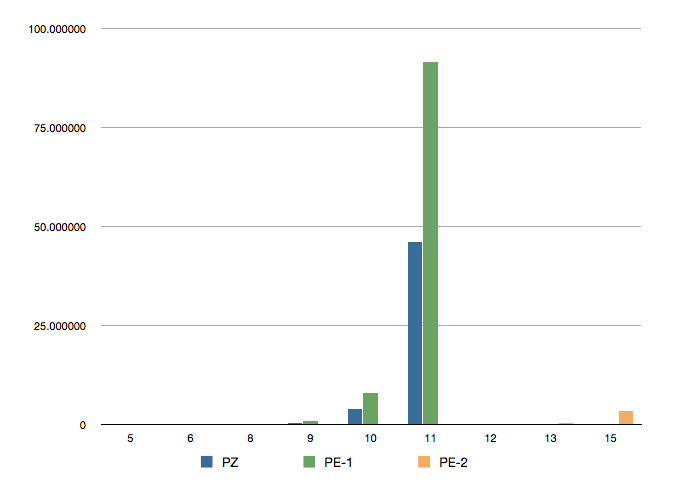
\includegraphics[scale=0.6]{wyk.png}
      \caption{Czas potrzebny do wyznaczenia optymalnego uszeregowania}
    \end{center}
  \end{figure}

  \newpage

  \section{Wnioski}
  \paragraph{}
  Po przeprowadzeniu analizy wyników można jednoznaczenie stwierdzić, iż druga procedura eliminacyjna
  jest nieporównywalnie szybsza od pierwszej jak i od przeglądu zupełnego.
  Wykres obrazuje jak duża jest różnica w czasie działania.
  Niewątpliwie wpływ na to ma wczesne odrzucanie gałęzi rozwiązań zastosowane w procedurze drugiej, które pozwala
  znacznie zmniejszyć ilość potrzebnych obliczeń.

  \paragraph{}
  Po wykonaniu profilowania kodu okazało się, że najwięcej czasu (ok 65-70\%) przeznaczone jest na obliczanie
  kosztu uszeregowania. Ma to szczególnie wpływ na pierwsza procedure eliminacyjna, która sprawdza koszt o wiele więcej razy
  niż przegląd zupełny, dlatego też w tym przypadku jest ona wolniejsza.



\end{document}